%\section{Anhang}\label{anhang}
\subsection{Konfigurationsdateien}
\begin{figure}[H]
	\lstinputlisting[caption={package.json für das GFB-Testprojekt}, label=lst:gfb-package]{lst/gfb/package.json}
\end{figure}

\begin{figure}[H]
	\lstinputlisting[caption={karma.conf.js für das GFB-Testprojekt}, label=lst:gfb-karma]{lst/gfb/karma.conf.js}
\end{figure}

\subsection{Komponententests}
\begin{figure}[H]
	\lstinputlisting[caption={test/spec/test\_spec.js}, label=lst:gfb-valid1]{test/spec/test_spec.js}
\end{figure}


\begin{figure}[H]
	\lstinputlisting[caption={test/spec/ngTest\_spec.js}, label=lst:gfb-valid2]{test/spec/ngTest_spec.js}
\end{figure}

\subsection{Code-Coverage}
\begin{figure}[H]
	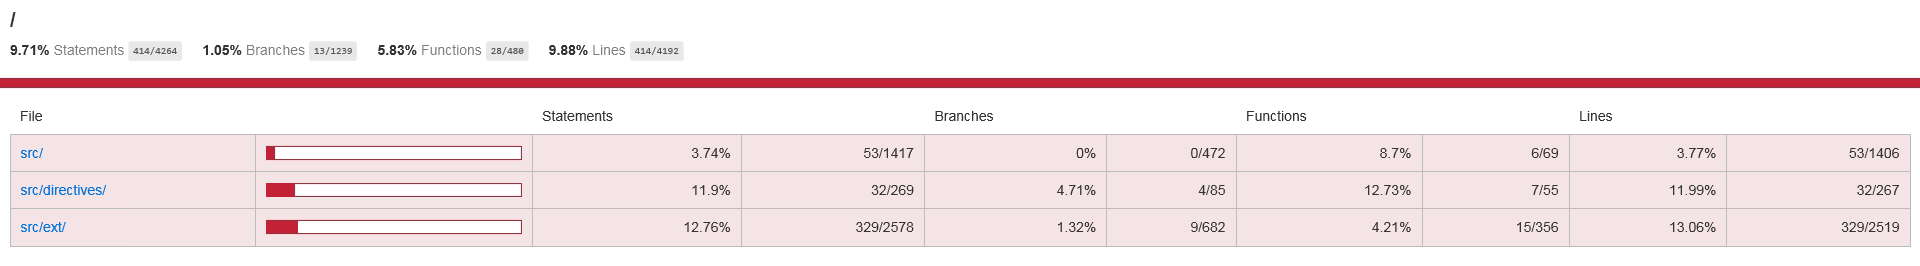
\includegraphics[width=\textwidth]{abb/code-cov-1.png}
	\caption{Übersichtsseite des Code-Coverage-Berichts im Browser}
	\label{abb:code-cov-1}
\end{figure}

\begin{figure}[H]
	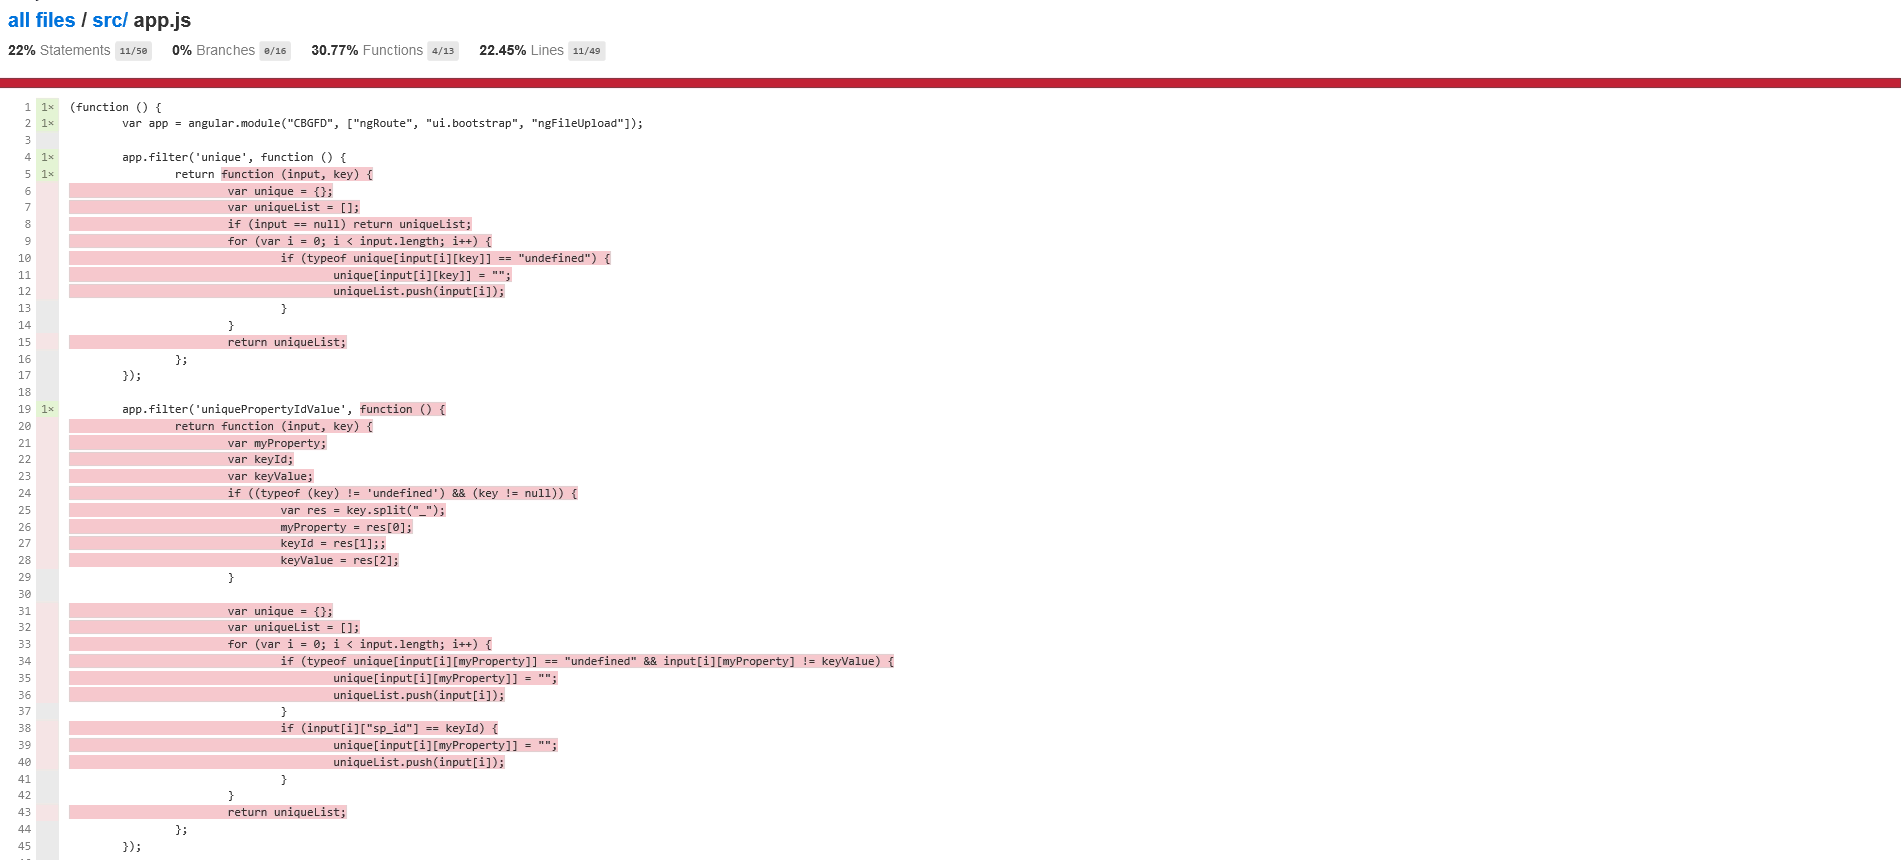
\includegraphics[width=\textwidth]{abb/code-cov-2.png}
	\caption[Detailseite des Code-Coverage-Berichts im Browser]{Detailseite des Code-Coverage-Berichts im Browser (Der abgebildete Quelltext ist Teil des GFB-Projekts und damit Eigentum der \domain)}
	\label{abb:code-cov-2}
\end{figure}